\fancyhead[C]{Section 15.6}
	\fancyhead[R]{\dayeighteen}
	
\iftoggle{questions}{
\begin{center}{\large \textbf{Math 2551 Worksheet: Mass and Moments}}
\end{center}

\begin{enumerate}
	
	\item Find the center of mass of a thin plate bounded by the line $y=1$ and the parabola $y=x^2$ if the density is $\delta(x,y)=y+1$.  \textit{Hint: Consider symmetry.}
	
	\begin{minipage}{0.6\textwidth}
		\item A solid of constant density $\delta(x,y,z)=2$ is bounded below by the plane $z=0$, on the sides by the elliptical cylinder $x^2+4y^2=4$, and above by the plane $z=2-x$.  Set up all of the necessary triple integrals to compute its center of mass.  You do not need to compute the center of mass.
	\end{minipage}
	\begin{minipage}{0.4\textwidth}
		\begin{center}
			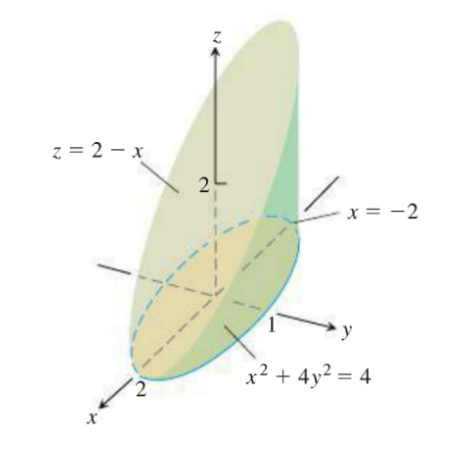
\includegraphics[scale=0.5]{15_6pic.PNG}
		\end{center}
	\end{minipage}
	
	{\large \textbf{Useful Formulas}}
	
	\begin{itemize}
		\item Mass: $M=\iiint_D \delta\ dV$ or $M=\iint_R \delta\ dA$\\
		
		\item First moments (2D plate): $M_{y}=\iint_R x\delta\ dA$,\ $M_{x}=\iint_R y\delta\ dA$\\
		
		\item Center of mass (2D plate): $(\bar{x},\bar{y})=\left(\dfrac{M_{y}}{M},\dfrac{M_{x}}{M}\right)$\\
		
		\item First moments (3D solid): $M_{yz}=\iiint_D x\delta\ dV$,\ $M_{xz}=\iiint_D y\delta\ dV$,\ $M_{xy}=\iiint_D z\delta\ dV$\\
		
		\item Center of mass (3D solid): $(\bar{x},\bar{y},\bar{z})=\left(\dfrac{M_{yz}}{M},\dfrac{M_{xz}}{M},\dfrac{M_{xy}}{M}\right)$\\
	\end{itemize}
%%%%%%
\end{enumerate}
}{}

\iftoggle{answers}
{
	\begin{center}{\large \textbf{Math 2551 Worksheet Answers: Mass and Moments}}
	\end{center}

\begin{enumerate}
		
	\item $(\bar{x},\bar{y})=\left(0,\dfrac{9}{14}\right)$

	\item Mass: $\int_{-2}^2\int_{-\sqrt{1-x^2/4}}^{\sqrt{1-x^2/4}} \int_0^{2-x} 2\ dz\ dy\ dx$
	
	$M_{yz}$: $\int_{-2}^2\int_{-\sqrt{1-x^2/4}}^{\sqrt{1-x^2/4}} \int_0^{2-x} 2x\ dz\ dy\ dx$
	
	$M_{xz}$: $\int_{-2}^2\int_{-\sqrt{1-x^2/4}}^{\sqrt{1-x^2/4}} \int_0^{2-x} 2y\ dz\ dy\ dx$
	
	$M_{xy}$: $\int_{-2}^2\int_{-\sqrt{1-x^2/4}}^{\sqrt{1-x^2/4}} \int_0^{2-x} 2z\ dz\ dy\ dx$
\end{enumerate}
}{}
\iftoggle{solutions}
{
Solutions go here in the same format.
}{}
